
\begin{frame}
	% Some examples of binary analysis methods are: 
	% binary debugging, which might be a little too manual in many cases;

	% Studying disassembly or decompiling using heuristics and meta data to
	% generate a higher level pseudocode;

	% fuzzing, generating different inputs and studying the outcome of the
	% program, like a crash;

	% Symbolic fuzzing, which we will get to.

	% All methods have their pros and cons and are applicable in different situations.
	% Binary debugging and studying disassembly or decompilation could be very
	% manual and burdenful for the analyst, but it could also give a very good
	% abstract understanding of the program.

	% Fuzzing is an automatic method and requires no interaction, but it doesn't
	% give any abstract understanding of the program. Only determining some
	% inputs satisfying user defined objectives. Like determining crashes,
	% detecting memory leaks and so on.

	% Another problem with fuzzing is the testcase generation. It is not trivial
	% how to generate test cases which effectively covers a large set of
	% execution paths so that no same paths are unneccessarily tested multiple
	% times, or reachable paths that were not explored.

	% The specific problem of test case generation is solved by symbolic fuzzing
	% which relies on symbolic execution.

	\begin{columns}[t]
		\begin{column}{0.5\textwidth}
			\begin{itemize}
				\item Binary debugging
				\item Disassembly
				\item Decompilation
				\item Fuzzing
				\item Symbolic fuzzing
			\end{itemize}
		\end{column}
		\begin{column}{0.5\textwidth}
			
\includegraphics[width=0.3\textwidth]{assets/GDB_Archer_Fish_by_Andreas_Arnez.svg.png}
			\footnote{\tiny by Andreas Arnez, \href{https://creativecommons.org/licenses/by-sa/3.0/us/deed.en}{CC BY-SA 3.0 us}}

			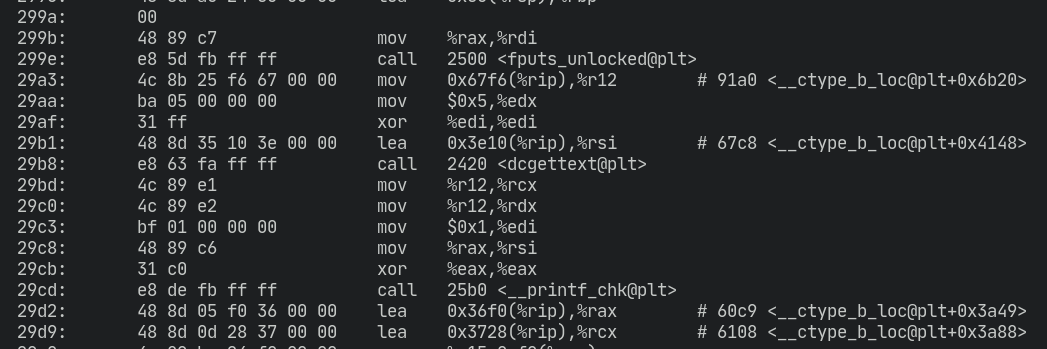
\includegraphics[width=\textwidth]{assets/disassembly.png}

			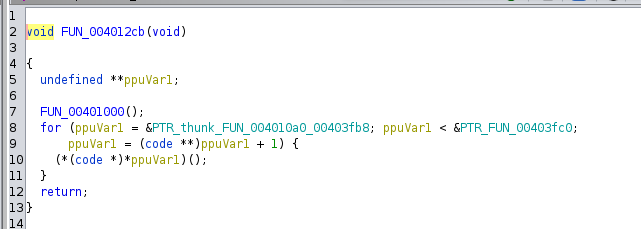
\includegraphics[width=\textwidth]{assets/decompil.png}

			\tiny{
				\begin{tikzpicture}

					\node [draw, fill=lightgray!80, minimum height=0.3cm]
					(first) {fuzz data generation};

					\node [draw, fill=lightgray!80, minimum height=0.3cm, right=0.2cm of first]
					(second) {execution};

					\node [draw, fill=lightgray!80, minimum height=0.3cm, below=0.2cm of second]
					(third) {analysis};

					\node [diamond, draw, fill=lightgray!80, minimum height=0.1cm, below=0.3cm of third]
					(fourth) {finished?};

					\node [draw, fill=lightgray!80, minimum height=0.3cm, right=0.2cm of fourth]
					(fifth) {report};

					\path [draw, -latex'] (first) to (second);
					\path [draw, -latex'] (second) to (third);
					\path [draw, -latex'] (third) to (fourth);
					\path [draw, -latex'] (fourth) to (fifth);
					\path [draw, -latex'] (fourth) -| (first);

				\end{tikzpicture}
			}
		\end{column}
	\end{columns}
\end{frame}
